\documentclass[aps,pra,twocolumn,superscriptaddress]{revtex4-2}

\usepackage{amsmath,amssymb,amsthm}
\usepackage{graphicx}
\usepackage{hyperref}
\usepackage{cleveref}

\newtheorem{proposition}{Proposition}
\newtheorem{corollary}{Corollary}
\newtheorem{conjecture}{Conjecture}
\newtheorem{definition}{Definition}

\begin{document}

\title{Zero-Noise Extrapolation as a Constrained Quantum Inverse Problem}

\author{The Son Nguyen}
\email{nguyensimon186@gmail.com}
\affiliation{Independent Researcher, Ho Chi Minh City, Vietnam}

\date{\today}

\begin{abstract}
Zero-noise extrapolation (ZNE) is one of the most widely used quantum error mitigation techniques, yet its theoretical foundations as an inference problem remain underdeveloped.
We formalize ZNE as a constrained inverse problem: recovering an unobserved noiseless expectation value from finite, noisy measurements at amplified noise levels.
We show that without function-class restrictions, the zero-noise limit is not identifiable from any finite set of observations (Proposition~1).
We establish that spectral bounds from the observable's eigenvalues provide physically valid constraints, and that post-hoc projection onto these bounds cannot increase pointwise error when the true value lies within the spectral interval (Proposition~2).
We introduce the \emph{ambiguity diameter}---the range of zero-noise values consistent with data, function class, and physical constraints---as a quantitative measure of identifiability.
Synthetic experiments illustrate that physical bounds reduce ambiguity diameter by up to $6.2\times$ in a degree-4 polynomial experiment at tolerance $\delta = 0.1$, and that a bias--ambiguity tradeoff governs model selection for ZNE.
All numerical results are synthetic and intended to illustrate the identifiability framework.
\end{abstract}

\maketitle

%% ============================================================
\section{Introduction}
\label{sec:intro}

Zero-noise extrapolation mitigates errors on noisy quantum processors by measuring expectation values at multiple amplified noise levels and extrapolating to the zero-noise limit~\cite{LiBenjamin2017,Temme2017}.
Since its introduction, ZNE has become a common error mitigation strategy due to its simplicity: no knowledge of the noise model is required, only the ability to amplify noise controllably.

Despite widespread use, ZNE is typically treated as a curve-fitting exercise.
This framing obscures a fundamental question: \emph{under what conditions is the zero-noise limit uniquely determined from finite noisy observations?}

We argue that ZNE is more naturally understood as a \textbf{constrained inverse problem} in the sense of Hadamard~\cite{Hadamard1902}: the noiseless expectation value is never directly observed, and must be inferred from indirect measurements subject to physical constraints.

%% ============================================================
\section{ZNE as a Constrained Inverse Problem}
\label{sec:inverse}

\subsection{Observation model}

Let $O$ be a Hermitian observable and $\mathcal{E}_\lambda$ a noise channel parameterized by scale factor $\lambda \geq 0$.
The observation model is:
\begin{equation}
y_i = f(\lambda_i) + \varepsilon_i, \quad i = 1, \ldots, n
\end{equation}
where $f(\lambda) = \mathrm{Tr}[\mathcal{E}_\lambda(\rho_{\mathrm{ideal}}) \, O]$ and $\varepsilon_i$ is shot noise.

\subsection{The inverse problem}

ZNE seeks $f(0)$ from $\{(\lambda_i, y_i)\}_{i=1}^n$, subject to:
\begin{itemize}
\item \textbf{Function class} $\mathcal{F}$: admissible response functions.
\item \textbf{Physical constraints} $\mathcal{C}$: spectral bounds $[\mu_{\min}, \mu_{\max}]$.
\item \textbf{Data consistency}: $\|f(\boldsymbol{\lambda}) - \mathbf{y}\|_\infty \leq \delta$.
\end{itemize}

%% ============================================================
\section{Non-Identifiability Without Assumptions}
\label{sec:nonident}

\begin{definition}[Ambiguity set]
\begin{equation}
\mathcal{A}(\mathbf{y}, \mathcal{F}, \mathcal{C}, \delta) = \left\{ f(0) \;\middle|\; f \in \mathcal{F}, \; f(0) \in \mathcal{C}, \; \|f(\boldsymbol{\lambda}) - \mathbf{y}\|_\infty \leq \delta \right\}
\end{equation}
\end{definition}

\begin{proposition}[Non-identifiability]
\label{prop:nonident}
Let $\lambda_1, \ldots, \lambda_n > 0$ be distinct.
For any observations $y_1, \ldots, y_n \in \mathbb{R}$ and any target $t \in \mathbb{R}$, there exists a polynomial $p$ of degree at most $n$ such that $p(\lambda_i) = y_i$ for all $i$ and $p(0) = t$.
\end{proposition}

\begin{proof}
The $n+1$ points $\{0, \lambda_1, \ldots, \lambda_n\}$ are distinct.
By Lagrange interpolation, there exists a unique polynomial of degree $\leq n$ taking prescribed values at $n+1$ distinct points.
\end{proof}

\begin{corollary}
For $\mathcal{F} = \mathcal{P}_n$ and $\mathcal{C} = \mathbb{R}$: $\mathcal{A}(\mathbf{y}, \mathcal{P}_n, \mathbb{R}, 0) = \mathbb{R}$.
\end{corollary}

%% ============================================================
\section{Physical Admissibility via Spectral Constraints}
\label{sec:spectral}

\begin{proposition}[Spectral validity]
\label{prop:spectral}
Let $O$ be Hermitian with eigenvalues $\mu_1, \ldots, \mu_m$.
For any density operator $\rho$:
\begin{equation}
\mu_{\min} \leq \mathrm{Tr}[\rho O] \leq \mu_{\max}
\end{equation}
\end{proposition}

\begin{proof}
$\mathrm{Tr}[\rho O] = \sum_j \mu_j p_j$ where $p_j = \langle e_j | \rho | e_j \rangle \geq 0$ and $\sum_j p_j = 1$.
A convex combination of real numbers lies within their range.
\end{proof}

\begin{corollary}[Projection reduces error]
For any estimate $\hat{f}$ and true value $f(0) \in [\mu_{\min}, \mu_{\max}]$:
$|\mathrm{proj}_{[\mu_{\min}, \mu_{\max}]}(\hat{f}) - f(0)| \leq |\hat{f} - f(0)|$.
\end{corollary}

%% ============================================================
\section{Ambiguity Diameter Experiments}
\label{sec:ambiguity}

We compute the ambiguity diameter numerically via linear programming.

\begin{figure}[t]
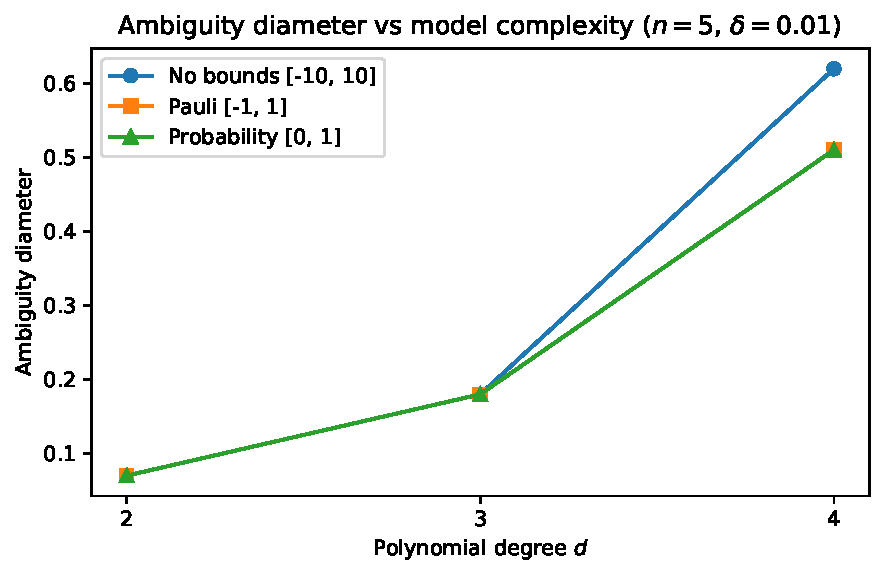
\includegraphics[width=\columnwidth]{../figures/ambiguity_degree_sweep.pdf}
\caption{Ambiguity diameter vs polynomial degree for $n=5$, $\delta=0.01$.
Physical bounds reduce ambiguity only when the function class is flexible (degree $\geq n-1$).}
\label{fig:degree_sweep}
\end{figure}

\begin{figure}[t]
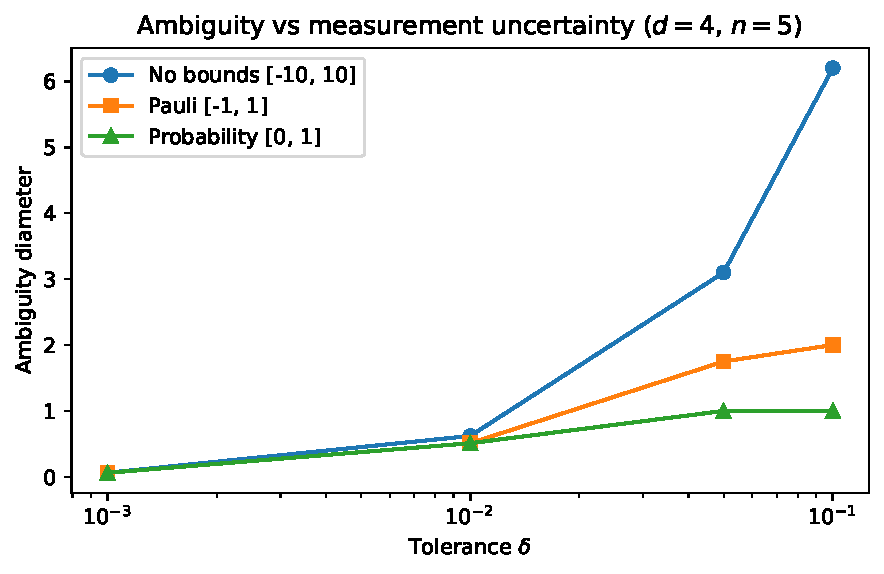
\includegraphics[width=\columnwidth]{../figures/delta_sensitivity.pdf}
\caption{Ambiguity diameter vs tolerance $\delta$ for degree 4, $n=5$.
Physical bounds cap ambiguity growth as measurement uncertainty increases.}
\label{fig:delta}
\end{figure}

\begin{figure}[t]
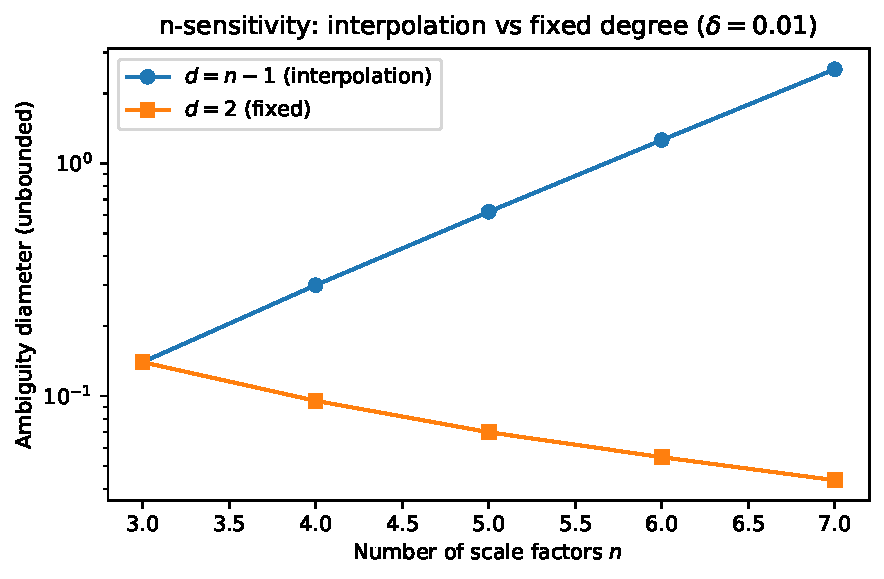
\includegraphics[width=\columnwidth]{../figures/n_sensitivity_interpolation_vs_fixed.pdf}
\caption{Ambiguity vs $n$: interpolation regime ($d=n-1$) shows growing ambiguity; fixed degree ($d=2$) shows shrinking ambiguity.
Identifiability depends on the ratio $n/(d+1)$, not $n$ alone.}
\label{fig:n_sensitivity}
\end{figure}

%% ============================================================
\section{Bias--Ambiguity Tradeoff}
\label{sec:tradeoff}

\begin{figure}[t]
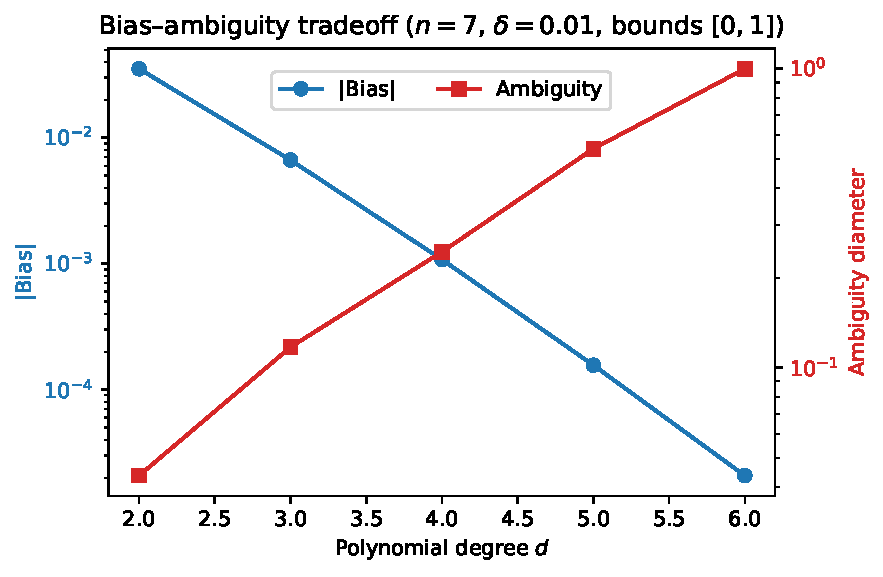
\includegraphics[width=\columnwidth]{../figures/bias_ambiguity_tradeoff.pdf}
\caption{Bias--ambiguity tradeoff for $n=7$, $\delta=0.01$, bounds $[0,1]$.
Lower degree reduces ambiguity but increases misspecification bias.
Model selection must balance these competing objectives.}
\label{fig:tradeoff}
\end{figure}

Identifiability alone is not accuracy.
A model can tightly identify the wrong value if misspecified.
The optimal degree balances bias against ambiguity, but depends on the unknown true response.

%% ============================================================
\section{Limitations}
\label{sec:limitations}

\begin{itemize}
\item All results use synthetic response functions. No quantum hardware is involved.
\item Only polynomial function classes are analyzed.
\item Tolerance $\delta$ is chosen manually; connection to shot budget is noted but not derived.
\item No proof that constrained optimization reduces MSE.
\item Single exponential response function; generalization is future work.
\end{itemize}

%% ============================================================
\begin{acknowledgments}
We thank the quantum error mitigation community for discussions on the interpretation of physically-bounded extrapolation.
\end{acknowledgments}

\bibliography{refs}

\end{document}
